%
% This document contains the chapter about noise waves.
%
% Copyright (C) 2003, 2004 Stefan Jahn <stefan@lkcc.org>
% Copyright (C) 2004 Michael Margraf <Michael.Margraf@alumni.TU-Berlin.DE>
%
% Permission is granted to copy, distribute and/or modify this document
% under the terms of the GNU Free Documentation License, Version 1.1
% or any later version published by the Free Software Foundation.
%

\chapter{Noise Waves}
%\addcontentsline{toc}{chapter}{Noise Waves}

\section{Definition}
%\addcontentsline{toc}{section}{Definition}

In microwave circuits described by scattering parameters, it is
advantageous to regard noise as noise waves \cite{Wedge}.  The noise
characteristics of an n-port is then defined completely by one
outgoing noise wave $\underline{b}_{noise,n}$ at each port (see 2-port
example in fig. \ref{fig:Sparam}) and the correlation between these
noise sources.  Therefore, mathematically, you can characterize a
noisy n-port by its $n\times n$ scattering matrix $(\underline{S})$
and its $n\times n$ noise wave correlation matrix $(\underline{C})$.

\begin{equation}
\begin{split}
(\underline{C}) =
\begin{pmatrix}
 \overline{\underline{b}_{noise,1}\cdot \underline{b}_{noise,1}^*} &
    \overline{\underline{b}_{noise,1}\cdot \underline{b}_{noise,2}^*} &
    \ldots & \overline{\underline{b}_{noise,1}\cdot \underline{b}_{noise,n}^*}\\
 \overline{\underline{b}_{noise,2}\cdot \underline{b}_{noise,1}^*} &
    \overline{\underline{b}_{noise,2}\cdot \underline{b}_{noise,2}^*} & \ldots &
    \overline{\underline{b}_{noise,2}\cdot \underline{b}_{noise,n}^*}\\
 \vdots & \vdots & \ddots & \vdots\\
 \overline{\underline{b}_{noise,n}\cdot \underline{b}_{noise,1}^*} &
    \overline{\underline{b}_{noise,n}\cdot \underline{b}_{noise,2}^*} &
    \ldots & \overline{\underline{b}_{noise,n}\cdot \underline{b}_{noise,n}^*}\\
\end{pmatrix}
\\ =
\begin{pmatrix}
  \underline{c}_{11} & \underline{c}_{12} & \ldots & \underline{c}_{1n}\\
  \underline{c}_{21} & \underline{c}_{22} & \ldots & \underline{c}_{2n}\\
  \vdots & \vdots & \ddots & \vdots\\
  \underline{c}_{n1} & \underline{c}_{n2} & \ldots & \underline{c}_{nn}\\
\end{pmatrix}
\end{split}
\label{eq:NoiseCs}
\end{equation}

Where $\overline{x}$ is the time average of $x$ and $\underline{x}^*$
is the conjugate complex of $\underline{x}$.  Noise correlation
matrices are hermitian matrices because the following equations hold.

\begin{equation}
\text{Im}\left(\underline{c}_{nn}\right) = \text{Im}\left(\overline{\left|b_{noise,n}\right|^2}\right) = 0
\end{equation}
\begin{equation}
\underline{c}_{nm} = \underline{c}_{mn}^*
\end{equation}

Where $\text{Im}(\underline{x})$ is the imaginary part of
$\underline{x}$ and $|\underline{x}|$ is the magnitude of
$\underline{x}$.

\begin{figure}[ht]
\begin{center}
\includegraphics[width=7cm]{sparam}
\end{center}
\caption{signal flow graph of a noisy 2-port}
\label{fig:Sparam}
\end{figure}
\FloatBarrier


\section{Noise Parameters}
%\addcontentsline{toc}{section}{Noise Parameters}

Having the noise wave correlation matrix, one can easily compute the
noise parameters \cite{Wedge}.  The following equations calculate them
with regard to port 1 (input) and port 2 (output).  (If one uses an
n-port and want to calculate the noise parameters regarding to other
ports, one has to replace the index numbers of S- and c-parameters
accordingly.  I.e. replace "1" with the number of the input port and
"2" with the number of the output port.)

\addvspace{12pt}

Noise figure:
\begin{equation}
F = 1 + \frac{\underline{c}_{22}}{k\cdot T_0\cdot |\underline{S}_{21}|^2}
\label{eq:nparamF}
\end{equation}
\begin{equation}
NF\,[\text{dB}]\, = 10\cdot\lg F
\end{equation}

\addvspace{12pt}

Optimal source reflection coefficient (normalized according to the input
port impedance):
\begin{equation}
\Gamma_{opt} = \eta_2\cdot\left( 1-\sqrt{1-\frac{1}{|\eta_2|^2}} \right)
\end{equation}
With
\begin{equation}
\eta_1 = \underline{c}_{11}\cdot |\underline{S}_{21}|^2
       - 2\cdot \text{Re}\left(\underline{c}_{12}\cdot\underline{S}_{21}\cdot\underline{S}_{11}^*\right)
       + \underline{c}_{22}\cdot|\underline{S}_{11}|^2
\end{equation}
\begin{equation}
\eta_2 = \frac{1}{2}\cdot\frac{\underline{c}_{22} + \eta_1}
              {\underline{c}_{22}\cdot\underline{S}_{11} - \underline{c}_{12}\cdot\underline{S}_{21}}
\end{equation}

\addvspace{12pt}

Minimum noise figure:
\begin{equation}
F_{min} = 1 + \frac{\underline{c}_{22} - \eta_1\cdot |\Gamma_{opt}|^2}
                   {k\cdot T_0\cdot |\underline{S}_{21}|^2\cdot (1+|\Gamma_{opt}|^2)}
\end{equation}
\begin{equation}
NF_{min} = 10\cdot \lg F_{min}
\end{equation}

\addvspace{12pt}

Equivalent noise resistance:
\begin{equation}
R_n = \frac{Z_{port,in}}{4\cdot k\cdot T_0}\cdot
      \left( \underline{c}_{11} - 2\cdot
      \text{Re}\left( \underline{c}_{12}\cdot\left( \frac{1+\underline{S}_{11}}{\underline{S}_{21}} \right)^*
      \right)\, + \underline{c}_{22}\cdot
      \left| \frac{1+\underline{S}_{11}}{\underline{S}_{21}} \right|^2 \right)
\label{eq:nparamRn}
\end{equation}
\begin{tabular}{ll}
With & \quad $Z_{port,in}$ internal impedance of input port\\
     & \quad Boltzmann constant $k = 1.380658\cdot 10^{-23}$ J/K\\
     & \quad standard temperature $T_0 = 290$K\\
\end{tabular}

\addvspace{12pt}

Calculating the noise wave correlation coefficients from the noise
parameters is straightforward as well.
\begin{equation}
\underline{c}_{11} = k\cdot T_{min}\cdot (|S_{11}|^2-1) + K_x\cdot |1-S_{11}\cdot\Gamma_{opt}|^2
\end{equation}
\begin{equation}
\underline{c}_{22} = |S_{21}|^2\cdot\left( k\cdot T_{min} + K_x\cdot|\Gamma_{opt}|^2 \right)
\end{equation}
\begin{equation}
\underline{c}_{12} =
\underline{c}_{21}^* = -S_{21}^*\cdot\Gamma_{opt}^*\cdot K_x + \frac{S_{11}}{S_{21}}\cdot\underline{c}_{22}
\end{equation}
with
\begin{equation}
K_x = \frac{4\cdot k\cdot T_0\cdot R_n}{Z_0\cdot|1+\Gamma_{opt}|^2}
\end{equation}


Once having the noise parameters, one can calculate the noise figure for
every source admittance $Y_S=G_S+j\cdot B_s$, source impedance
$Z_S=R_S+j\cdot X_s$, or source reflection coefficient $r_S$.

\begin{align}
  F & = \frac{SNR_{in}}{SNR_{out}} = \frac{T_{equi}}{T_0} + 1\\
    & = F_{min} + \frac{G_n}{R_S}\cdot\left( (R_S-R_{opt})^2 + (X_S-X_{opt})^2 \right)\\
    & = F_{min} + \frac{G_n}{R_S}\cdot\left| \underline{Z}_S - \underline{Z}_{opt} \right| ^2\\
    & = F_{min} + \frac{R_n}{G_S}\cdot\left( (G_S-G_{opt})^2 + (B_S-B_{opt})^2 \right)\\
    & = F_{min} + \frac{R_n}{G_S}\cdot\left| \underline{Y}_S - \underline{Y}_{opt} \right| ^2\\
    & = F_{min} + 4\cdot\frac{R_n}{Z_0}\cdot\frac{\left| \underline{\Gamma}_{opt}-\underline{r}_S\right| ^2}
                  {\left( 1-|\underline{r}_S|^2\right)\cdot\left| 1+\underline{\Gamma}_{opt}\right| ^2}
\end{align}

Where $SNR_{in}$ and $SNR_{out}$ are the signal to noise ratios at the
input and output, respectively, $T_{equi}$ is the equivalent (input)
noise temperature.  Note that $G_n$ does not equal $1/R_n$.

\addvspace{12pt}

All curves with constant noise figures are circles (in all planes,
i.e. impedance, admittance and reflection coefficient).  A circle in
the reflection coefficient plane has the following parameters.

\addvspace{12pt}

center point:
\begin{equation}
\underline{r}_{center} = \frac{\Gamma_{opt}}{1+N}
\end{equation}
radius:
\begin{equation}
R = \frac{\sqrt{N^2 + N\cdot(1-|\Gamma_{opt}|^2)}}{1+N}
\end{equation}
with
\begin{equation}
N = \frac{Z_0}{4\cdot R_n}\cdot (F-F_{min})\cdot |1+\Gamma_{opt}|^2
\end{equation}


\section{Noise Wave Correlation Matrix in CAE}
%\addcontentsline{toc}{section}{Noise Wave Correlation Matrix in CAE}

Due to the similar concept of S parameters and noise correlation
coefficients, the CAE noise analysis can be performed quite alike the
S parameter analysis (section \ref{sec:SparameterCAE}). As each step
uses the S parameters to calculate the noise correlation matrix, the
noise analysis is best done step by step in parallel with the S
parameter analysis.  Performing each step is as follows: We have the
noise wave correlation matrices ( $(\underline{C})$, $(\underline{D})$
) and the S parameter matrices ( $(\underline{S})$, $(\underline{T})$
) of two arbitrary circuits and want to know the correlation matrix of
the special circuit resulting from connecting two circuits at one
port.

\begin{figure}[ht]
\begin{center}
\includegraphics[width=\linewidth]{nconnect}
\end{center}
\caption{connecting two noisy circuits, scheme (left) and signal flow graph (right)}
\label{fig:nconnect}
\end{figure}
\FloatBarrier

An example is shown in fig. \ref{fig:nconnect}.  What we have to do is
to transform the inner noise waves $\underline{b}_{noise,k}$ and
$\underline{b}_{noise,l}$ to the open ports.  Let us look upon the
example.  According to the signal flow graph the resulting noise wave
$\underline{b}_{noise,i}'$ writes as follows:
\begin{equation}
\underline{b}_{noise,i}' = \underline{b}_{noise,i} +
    \underline{b}_{noise,k}\cdot
            \frac{\underline{T}_{ll}\cdot \underline{S}_{ik}}{1-\underline{S}_{kk}\cdot\underline{T}_{ll}} +
    \underline{b}_{noise,l}\cdot
            \frac{\underline{S}_{ik}}{1-\underline{S}_{kk}\cdot\underline{T}_{ll}}
\label{eq:bnoiseI}
\end{equation}
The noise wave $\underline{b}_{noise,j}$ does not contribute to
$\underline{b}_{noise,i}'$, because no path leads to port $i$.
Calculating $\underline{b}_{noise,j}'$ is quite alike:
\begin{equation}
\underline{b}_{noise,j}' = \underline{b}_{noise,j} +
    \underline{b}_{noise,l}\cdot
            \frac{\underline{T}_{jl}\cdot \underline{S}_{kk}}{1-\underline{S}_{kk}\cdot\underline{T}_{ll}} +
    \underline{b}_{noise,k}\cdot
            \frac{\underline{T}_{jl}}{1-\underline{S}_{kk}\cdot\underline{T}_{ll}}
\label{eq:bnoiseJ}
\end{equation}

Now we can derive the first element of the new noise correlation
matrix by multiplying eq. \eqref{eq:bnoiseI} with eq. \eqref{eq:bnoiseJ}.
\begin{equation}
\begin{split}
\underline{c}_{ij}' = & \quad \overline{\underline{b}_{noise,i}'\cdot\underline{b}_{noise,j}'^*} \\
 = & \quad\; \overline{\underline{b}_{noise,i}\cdot\underline{b}_{noise,j}^*} \\
 & + \overline{\underline{b}_{noise,i}\cdot\underline{b}_{noise,l}^*}\cdot
       \left( \frac{\underline{T}_{jl}\cdot \underline{S}_{kk}}{1-\underline{S}_{kk}\cdot\underline{T}_{ll}}
                \right)^* +
       \overline{\underline{b}_{noise,i}\cdot\underline{b}_{noise,k}^*}\cdot
       \left( \frac{\underline{T}_{jl}}{1-\underline{S}_{kk}\cdot\underline{T}_{ll}} \right) ^* \\
 & + \overline{\underline{b}_{noise,k}\cdot\underline{b}_{noise,j}^*}\cdot
       \frac{\underline{T}_{ll}\cdot \underline{S}_{ik}}{1-\underline{S}_{kk}\cdot\underline{T}_{ll}} \\
 & + \overline{\underline{b}_{noise,k}\cdot\underline{b}_{noise,l}^*}\cdot
       \frac{\underline{T}_{ll}\cdot \underline{S}_{ik}\cdot \underline{T}_{jl}^* \cdot\underline{S}_{kk}^*}
            {| 1-\underline{S}_{kk}\cdot\underline{T}_{ll} |^2} +
       \overline{\underline{b}_{noise,k}\cdot\underline{b}_{noise,k}^*}\cdot
       \frac{\underline{T}_{ll}\cdot \underline{S}_{ik}\cdot \underline{T}_{jl}^*}
            {| 1-\underline{S}_{kk}\cdot\underline{T}_{ll} |^2} \\
 & + \overline{\underline{b}_{noise,l}\cdot\underline{b}_{noise,j}^*}\cdot
       \frac{\underline{S}_{ik}}{1-\underline{S}_{kk}\cdot\underline{T}_{ll}} \\
 & + \overline{\underline{b}_{noise,l}\cdot\underline{b}_{noise,l}^*}\cdot
       \frac{\underline{S}_{ik}\cdot \underline{T}_{jl}^*\cdot \underline{S}_{kk}^*}
            {| 1-\underline{S}_{kk}\cdot\underline{T}_{ll} |^2} +
       \overline{\underline{b}_{noise,l}\cdot\underline{b}_{noise,k}^*}\cdot
       \frac{\underline{S}_{ik}\cdot \underline{T}_{jl}^*}
            {| 1-\underline{S}_{kk}\cdot\underline{T}_{ll} |^2}
\end{split}
\end{equation}
The noise waves of different circuits are uncorrelated and therefore
their time average product equals zero (e.g.
$\overline{\underline{b}_{noise,i}\cdot\underline{b}_{noise,j}^*} =
0$).  Thus, the final result is:
\begin{equation}
\begin{split}
\underline{c}_{ij}' = (\underline{c}_{ji}')^* =
   (\underline{c}_{kk}\cdot\underline{T}_{ll} + \underline{d}_{ll}\cdot\underline{S}_{kk}^*)\cdot
   \frac{\underline{S}_{ik}\cdot\underline{T}_{jl}^*}{|1-\underline{S}_{kk}\cdot\underline{T}_{ll}|^2}
\\ + \;\underline{c}_{ik}\cdot
     \left(\frac{\underline{T}_{jl}}{1-\underline{S}_{kk}\cdot\underline{T}_{ll}}\right)^*
   + \underline{d}_{lj}\cdot
     \frac{\underline{S}_{ik}}{1-\underline{S}_{kk}\cdot\underline{T}_{ll}}
\end{split}
\end{equation}


All other cases of connecting circuits can be calculated the same way
using the signal flow graph.  The results are listed below.

\addvspace{12pt}

If index $i$ and $j$ are within the same circuit, it results in
fig. \ref{fig:nconnect2}.  The following formula holds:

\begin{equation}
\begin{split}
\underline{c}_{ij}' = (\underline{c}_{ji}')^* = \underline{c}_{ij} +
   (\underline{c}_{kk}\cdot|\underline{T}_{ll}|^2 + \underline{d}_{ll})\cdot
   \frac{\underline{S}_{ik}\cdot\underline{S}_{jk}^*}{|1-\underline{S}_{kk}\cdot\underline{T}_{ll}|^2}
\\ + \;\underline{c}_{ik}\cdot
     \left(\frac{\underline{T}_{ll}\cdot\underline{S}_{jk}}
                {1-\underline{S}_{kk}\cdot\underline{T}_{ll}}\right)^*
   + \underline{c}_{kj}\cdot
     \frac{\underline{T}_{ll}\cdot\underline{S}_{ik}}{1-\underline{S}_{kk}\cdot\underline{T}_{ll}}
\end{split}
\end{equation}
This equation is also valid, if $i$ equals $j$.

\begin{figure}[ht]
\begin{center}
\includegraphics[width=7cm]{nconnect2}
\end{center}
\caption{connecting two noisy circuits}
\label{fig:nconnect2}
\end{figure}
\FloatBarrier


If the connected ports $k$ and $l$ are from the same circuit, the
following equations must be applied (see also
fig. \ref{fig:nconnect3}) to obtain the new correlation matrix
coefficients.

\begin{equation}
M = (1-\underline{S}_{kl})\cdot(1-\underline{S}_{lk}) - \underline{S}_{kk}\cdot\underline{S}_{ll}
\end{equation}
\begin{equation}
K_1 = \frac{\underline{S}_{il}\cdot(1-\underline{S}_{lk}) + \underline{S}_{ll}\cdot\underline{S}_{ik}} {M}
\end{equation}
\begin{equation}
K_2 = \frac{\underline{S}_{ik}\cdot(1-\underline{S}_{kl}) + \underline{S}_{kk}\cdot\underline{S}_{il}} {M}
\end{equation}
\begin{equation}
K_3 = \frac{\underline{S}_{jl}\cdot(1-\underline{S}_{lk}) + \underline{S}_{ll}\cdot\underline{S}_{jk}} {M}
\end{equation}
\begin{equation}
K_4 = \frac{\underline{S}_{jk}\cdot(1-\underline{S}_{kl}) + \underline{S}_{kk}\cdot\underline{S}_{jl}} {M}
\end{equation}

\begin{equation}
\begin{split}
\underline{c}_{ij}' = \underline{c}_{ij} &+ \underline{c}_{kj}\cdot K_1 + \underline{c}_{lj}\cdot K_2
   + K_3^*\cdot(\underline{c}_{ik} + \underline{c}_{kk}\cdot K_1 + \underline{c}_{lk}\cdot K_2) + \\
    &K_4^*\cdot(\underline{c}_{il} + \underline{c}_{kl}\cdot K_1 + \underline{c}_{ll}\cdot K_2)
\end{split}
\end{equation}
These equations are also valid if $i$ equals $j$.

\begin{figure}[ht]
\begin{center}
\includegraphics[width=4.5cm]{nconnect3}
\end{center}
\caption{connection within a noisy circuits}
\label{fig:nconnect3}
\end{figure}
\FloatBarrier

The absolute values of the noise correlation coefficients are very
small.  To achieve a higher numerical precision, it is recommended to
normalize the noise matrix with $k\cdot T_0$. After the simulation
they do not have to be denormalized, because the noise parameters can
be calculated by using equation \eqref{eq:nparamF} to
\eqref{eq:nparamRn} and omitting all occurrences of $k\cdot T_0$.

\addvspace{12pt}

The transformer concept to deal with different port impedances and
with differential ports (as described in section \ref{sec:diffSParam})
can also be applied to this noise analysis.


\section{Noise Correlation Matrix Transformations}
%\addcontentsline{toc}{section}{Noise Correlation Matrix Transformations}

The noise wave correlation matrix of a passive linear circuit
generating thermal noise can simply be calculated using Bosma's theorem.
The noise wave correlation matrices of active devices can be
determined by forming the noise current correlation matrix and then
transforming it to the equivalent noise wave correlation matrix.

\addvspace{12pt}

The noise current correlation matrix (also called the admittance
representation) $\underline{C}_Y$ is an $n \times n$ matrix.
\begin{equation}
\underline{C}_Y =
\begin{pmatrix}
\overline{\underline{i}_{1}\cdot \underline{i}_{1}^*} &
    \overline{\underline{i}_{1}\cdot \underline{i}_{2}^*} &
    \ldots & \overline{\underline{i}_{1}\cdot \underline{i}_{n}^*}\\
 \overline{\underline{i}_{2}\cdot \underline{i}_{1}^*} &
    \overline{\underline{i}_{2}\cdot \underline{i}_{2}^*} & \ldots &
    \overline{\underline{i}_{2}\cdot \underline{i}_{n}^*}\\
 \vdots & \vdots & \ddots & \vdots\\
 \overline{\underline{i}_{n}\cdot \underline{i}_{1}^*} &
    \overline{\underline{i}_{n}\cdot \underline{i}_{2}^*} &
    \ldots & \overline{\underline{i}_{n}\cdot \underline{i}_{n}^*}\\
\end{pmatrix}
=
\begin{pmatrix}
  \underline{c}_{11} & \underline{c}_{12} & \ldots & \underline{c}_{1n}\\
  \underline{c}_{21} & \underline{c}_{22} & \ldots & \underline{c}_{2n}\\
  \vdots & \vdots & \ddots & \vdots\\
  \underline{c}_{n1} & \underline{c}_{n2} & \ldots & \underline{c}_{nn}\\
\end{pmatrix}
\end{equation}

This definition is very likely the one made by eq. \eqref{eq:NoiseCs}.
The matrix has the same properties as well.  Because in most
transistor models the noise behaviour is expressed as the sum of
effects of noise current sources it is easier to form this matrix
representation.

\subsection{Forming the noise current correlation matrix}
%\addcontentsline{toc}{subsection}{Forming the noise current correlation matrix}

Each element in the diagonal matrix is equal to the sum of the noise
current of each element connected to the corresponding node.  So the
first diagonal element is the sum of noise currents connected to node
1, the second diagonal element is the sum of noise currents connected
to node 2, and so on.

\addvspace{12pt}

The off diagonal elements are the negative noise current of the
element connected to the pair of corresponding node.  Therefore a
noise current source between nodes 1 and 2 goes into the matrix at
location (1,2) and locations (2,1).

\addvspace{12pt}

If a noise current source is grounded, it will only have contribute to
one entry in the noise correlation matrix -- at the appropriate
location on the diagonal.  If it is ungrounded it will contribute to
four entries in the matrix -- two diagonal entries (corresponding to
the two nodes) and two off-diagonal entries.

\begin{figure}[ht]
\begin{center}
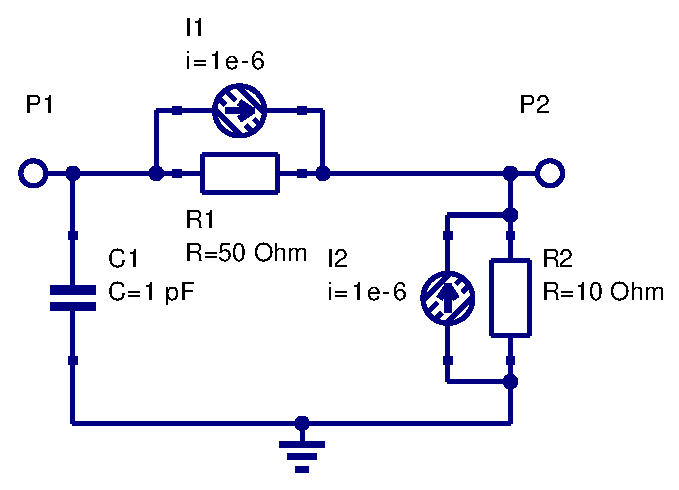
\includegraphics[width=8cm]{CYexample}
\end{center}
\caption{example circuit applied to noise analysis}
\label{fig:CYexample}
\end{figure}
\FloatBarrier

Once having defined the spectral noise current densities of the noise
currents within a transistor model the above rules for forming the
$\underline{C}_Y$ matrix can be applied to the example circuit
depicted in fig. \ref{fig:CYexample}.  The noise current
correlation matrix is accordingly
\begin{equation}
\underline{C}_Y =
\begin{bmatrix}
+\overline{i_1^2} & -\overline{i_1^2}\\
-\overline{i_1^2} & \overline{i_1^2} + \overline{i_2^2}\\
\end{bmatrix}
\end{equation}

\subsection{Transformations}
%\addcontentsline{toc}{subsection}{Transformations}
\label{sec:noiseTrans}

There are three usable noise correlation matrix representations for
multiport circuits.

\begin{itemize}
\item admittance representation $\underline{C}_Y$ - based on noise currents
\item impedance representation $\underline{C}_Z$ - based on noise voltages
\item wave representation $\underline{C}_S$ - based on noise waves
\end{itemize}

According to Scott W. Wedge and David B. Rutledge \cite{Wedge} the
transformations between these representations write as follows.

\begin{center}
\setlength{\fboxsep}{3pt}
\begin{tabular}{|r|c|c|c|}
\hline
&
\setlength{\fboxrule}{0pt}
\fbox{$\underline{C}_Y$}  & $\underline{C}_Z$ & $\underline{C}_S$\\
\hline
$\underline{C}_Y$ & $\underline{C}_Y$ & $Y\cdot \underline{C}_Z\cdot Y^{+}$ &
\setlength{\fboxrule}{0pt}
\fbox{$\left(E + Y\right)\cdot \underline{C}_S\cdot \left(E + Y\right)^{+}$}\\
\hline
$\underline{C}_Z$ & $Z\cdot \underline{C}_Y\cdot Z^{+}$ & $\underline{C}_Z$ &
\setlength{\fboxrule}{0pt}
\fbox{$\left(E + Z\right)\cdot \underline{C}_S\cdot \left(E + Z\right)^{+}$}\\
\hline
$\underline{C}_S$ &
\setlength{\fboxrule}{0pt}
\fbox{$\dfrac{1}{4} \left(E + S\right)\cdot \underline{C}_Y\cdot \left(E + S\right)^{+}$} & $\dfrac{1}{4} \left(E - S\right)\cdot \underline{C}_Z\cdot \left(E - S\right)^{+}$ & $\underline{C}_S$\\
\hline
\end{tabular}
\end{center}

The signal as well as correlation matrices in impedance and admittance
representations are assumed to be normalized in the above table.  $E$
denotes the identity matrix and the $ ^{+}$ operator indicates the
transposed conjugate matrix (also called adjoint or adjugate).

\addvspace{12pt}

Each noise correlation matrix transformation requires the appropriate
signal matrix representation which can be obtained using the formulas
given in section \ref{sec:SparameterConversion} on page
\pageref{sec:SparameterConversion}.

\section{Noise Wave Correlation Matrix of Components}
%\addcontentsline{toc}{section}{Noise Wave Correlation Matrix of Components}

Many components do not produce any noise.  Every element of their
noise correlation matrix therefore equals exactly zero.  Examples are
lossless, passive components, i.e. capacitors, inductors,
transformers, circulators, phase shifters.  Furthermore ideal voltage
and current sources (without internal resistance) as well as gyrators
also do not produce any noise.

\addvspace{12pt}

If one wants to calculate the noise wave correlation matrix of a
component, the most universal method is to take noise voltages and
noise currents and then derive the noise waves by the use of equation
\eqref{equ:waves}.  However, this can be very difficult.

\addvspace{12pt}

A passive, linear circuit produces only thermal noise and thus its
noise waves can be calculated with Bosma's theorem (assuming
thermodynamic equilibrium).

\begin{equation}
\label{eqn:bosma}
(\underline{C}) = k\cdot T\cdot \left( (\underline{E}) - (\underline{S})\cdot(\underline{S})^{*T} \right)
\end{equation}
with $(\underline{S})$ being the S parameter matrix and $(\underline{E})$ identity matrix.
Of course, this theorem can also be written with impedance and admittance representation
of the noise correlation matrix:
\begin{equation}
\underline{C}_Z = 4\cdot k\cdot T\cdot \text{Re}(\underline{Z})
\end{equation}
\begin{equation}
\underline{C}_Y = 4\cdot k\cdot T\cdot \text{Re}(\underline{Y})
\end{equation}
